% report-demo.tex：一頁有「圖」、有「表」、有「引用」的報告範本。
% 同一個專案（或同一個資料夾）要有三個檔：這個檔、figure-demo.png、refs.bib。
% Overleaf：三個檔都上傳，Compiler 選 XeLaTeX，按 Recompile。
% 本機：xelatex report-demo → bibtex report-demo → xelatex report-demo → xelatex report-demo
\documentclass[11pt,a4paper]{article}
\usepackage{xeCJK}
\IfFontExistsTF{Noto Serif CJK TC}{\setCJKmainfont{Noto Serif CJK TC}}{\IfFontExistsTF{Microsoft JhengHei}{\setCJKmainfont{Microsoft JhengHei}}{\setCJKmainfont{Songti TC}}}
\usepackage[margin=2cm]{geometry}
\usepackage{graphicx}
\renewcommand{\figurename}{圖}
\renewcommand{\tablename}{表}
\renewcommand{\refname}{參考文獻}

\title{每週編譯錯誤數的變化}
\author{你的稱呼（可用化名）}
\date{}

\begin{document}
\maketitle

\section{我想了解的問題}
剛學 LaTeX 時，每次編譯都會遇到錯誤。練習八週之後，錯誤有沒有變少？下面用的是示範資料，不是真實量測。

\section{一張圖}
圖~\ref{fig:errors} 是用 gnuplot 讀資料檔畫出來的。兩組的錯誤數都逐週下降。

\begin{figure}[htbp]
  \centering
  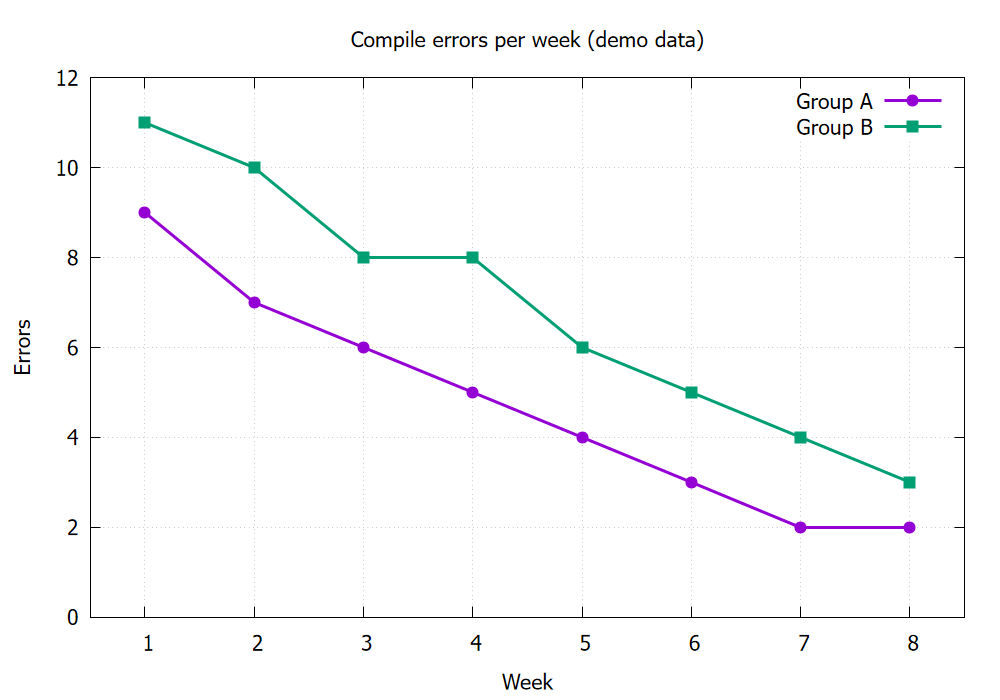
\includegraphics[width=0.45\linewidth]{figure-demo.png}
  \caption{每週編譯錯誤數（示範資料）。}
  \label{fig:errors}
\end{figure}

\section{一張表}
表~\ref{tab:errors} 列出第 1、4、8 週的數字。表號和圖號一樣，由 LaTeX 自己編。

\begin{table}[htbp]
  \centering
  \caption{三個時間點的編譯錯誤數（示範資料）。}
  \label{tab:errors}
  \begin{tabular}{ccc}
    \hline
    週次 & A 組 & B 組 \\
    \hline
    1 & 9 & 11 \\
    4 & 5 & 8 \\
    8 & 2 & 3 \\
    \hline
  \end{tabular}
\end{table}

\section{一篇文獻}
有人帶著練習，是不是比自己摸索有效？Su 等人做過有對照組的訓練研究 \cite{Su2021}。引用之前要回原文核對題名、作者與年份。

\bibliographystyle{plain}
\bibliography{refs}
\end{document}
